\subsection{Hàm đa thức}

\ % Lùi đầu dòng

Một dạng hàm quen thuộc, được giới thiệu trong chương trình học trung học phổ thông, là đa thức, thông thường được biểu diễn dưới dạng $$f(x)=P_n(x)=\sum_{i = 0}^n a_i x^i = a_nx^n + a_{n-1}x^{n-1} + \cdots + a_1x + a_0$$ với $n$ là một số nguyên không âm, $a_i$ là các số thực, gọi là các \emph{hệ số}, với mọi $i$ nguyên nằm trong đoạn $[0, n]$ và $a_n \neq 0$. Khi này, $n$ được gọi là \emph{bậc} của đa thức\label{def:ham_so_mot_bien:da_thuc:da_thuc}. Mọi giá trị $x \in \mathbb{R}$ đều thuộc tập xác định của hàm đa thức $f(x)$. Ví dụ:
\begin{itemize}
   \item $f(x) = 2x^2 + 3x + 1$ là một đa thức bậc $2$ với các hệ số $a_2 = 2$, $a_1 = 3$, $a_0 = 1$;
   \item $g(y) = y^3 - 4y$ là một đa thức bậc $3$ với các hệ số $b_3 = 1$, $b_2 = 0$, $b_1 = -4$, $b_0 = 0$;
   \item $h(z) = 5$ là một đa thức bậc $0$ với hệ số $c_0 = 5$;
\end{itemize}
Tính toán một số giá trị mẫu:
\begin{itemize}
   \item $p(1) = 7 \cdot 1^4 - 2 \cdot 1^2 + 9 = 14$ với $q(t)= 7t^4 - 2t^2 + 9$ là một đa thức bậc $4$ với các hệ số $d_4 = 7$, $d_3 = 0$, $d_2 = -2$, $d_1 = 0$, $d_0 = 9$;
   \item $q(2) = -3 \cdot 2 + 8 = 2$ với $q(r) = -3r + 8$ là một đa thức bậc $1$ với các hệ số $e_1 = -3$, $e_0 = 8$.
\end{itemize}
Khi đa thức có bậc bằng $0$, hay $f = P_0 = a_0$, thì được gọi là \emph{đa thức hằng} hay \emph{hàm hằng}. Một trường hợp đặc biệt là khi $f = 0$ (hay $f(x) = 0$ với mọi $x$). Nếu hàm này là đa thức, theo định nghĩa, hàm này chỉ có duy nhất hệ số đầu $a_0 = 0$. Tuy nhiên, cũng theo định nghĩa thì hệ số đầu phải khác $0$. Vì vậy, hàm không có bậc và không được gọi là đa thức. Nhưng, do hàm nhận giá trị cố định với mọi $x$ nên vẫn được gọi là hàm hằng \footnote{Đa số những nhà toán học không coi $f = 0$ là đa thức bậc $0$ do nhiều tính chất của đa thức bị phá vỡ khi gặp trường hợp này. Tuy nhiên, nhiều người vẫn coi $f = 0$ là đa thức không có bậc. Trong tài liệu này, tác giả không coi $0$ là đa thức, nhưng vẫn coi là hàm hằng.}.

\exercise Phác thảo đồ thị của những hàm sau:
\begin{multicols}{2}
   \begin{enumerate}
      \item $f(x) = x + 2$; 
      \item $f(x) = x^2 + 2x + 3$;
      \item $f(x) = -2x^2 + 5x - 6$;
      \item $f(x) = x^3 - 9x^2 + 24x - 16$;
      \item $f(x) = 2$;
      \item $f(x) = 36x^4 + 28x^3 - 3x^2 - 6x - 1$;
      \item $f(x) = -x^6 + x^2 - 4x - 2$;
      \item $f(x) = -x^7 + x$.
   \end{enumerate}
\end{multicols}

\solution

Bạn đọc có thể dùng những phần mềm vẽ đồ thị để nhanh chóng có hình vẽ. Tuy nhiên, nếu không có thiết bị điện tử thì bạn đọc vẫn có thể vẽ đồ thị bằng giấy và bút bằng cách lấy nhiều điểm ví dụ cho $x$ và tính toán giá trị $f(x)$ và sau đó nối chúng lại với nhau.

Bạn đọc có thể để ý rằng là không phải lúc nào cũng đặt gốc tọa độ ở vị trí chính giữa và tỉ lệ xích trên hai trục không phải là giống nhau. Trong nhiều trường hợp, việc ép đặt gốc ở giữa và giữ tỉ lệ giống nhau trên các trục sẽ làm cho đồ thị lệch ra khỏi khu vực vẽ. Điều quan trọng nhất của những bài vẽ đồ thị trong vật lí không chỉ là căn ke chính xác vị trí từng điểm, mà còn là nhận ra được dáng điệu của đồ thị và vị trí tương đối giữa các điểm trên đồ thị đó. Qua đó, chúng ta rút ra được những tính chất toán học cần thiết để phục vụ những yêu cầu cụ thể trong bài tập ứng dụng.

Dưới đây là đồ thị của các hàm đa thức trong bài:

\begin{multicols}{2}
   \begin{figure}[H]
      \centering
      \fbox{
         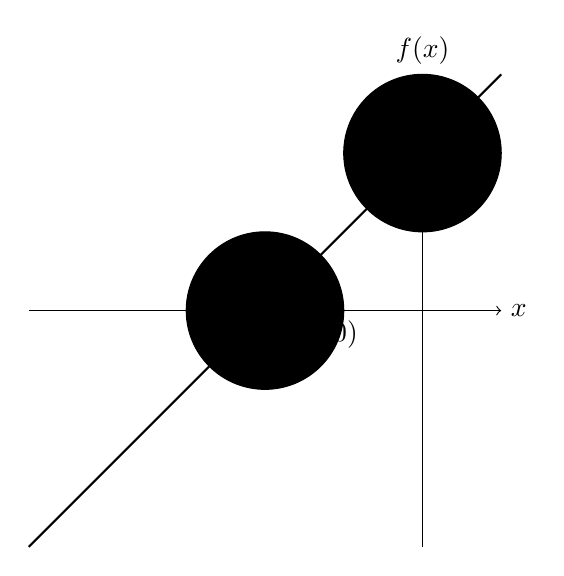
\begin{tikzpicture}
            \draw[->] (-5, 0) -- (1, 0) node[right] {$x$};
            \draw[->] (0, -3) -- (0, 3) node[above] {$f(x)$};
            \draw[thick] plot[domain=-5:1] (\x, {\x + 2});
            \filldraw (0, 2) circle (\pointSize) node[below right] {$\left(0; 2\right)$};
            \filldraw (-2, 0) circle (\pointSize) node[below right] {$\left(-2; 0\right)$};
         \end{tikzpicture}
      }
      \caption{Đồ thị của hàm $f(x) = x + 2$}
      \label{fig:ham_so:ham_da_thuc:x_2}
   \end{figure}
   
   \begin{figure}[H]
      \centering
      \fbox{
         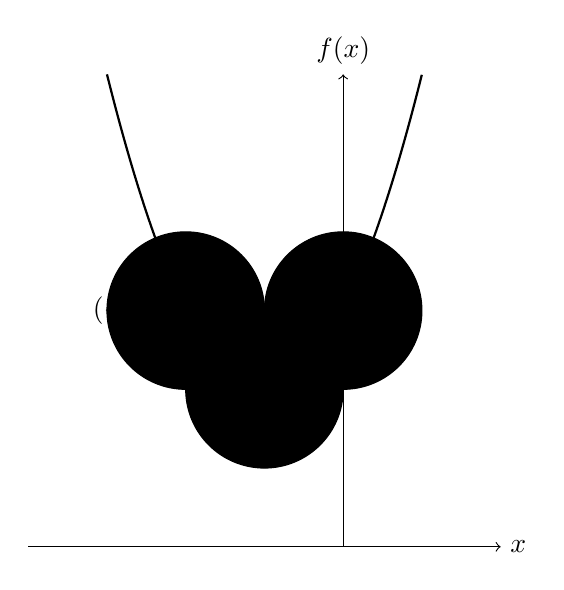
\begin{tikzpicture}
            \draw[->] (-4, 0) -- (2, 0) node[right] {$x$};
            \draw[->] (0, 0) -- (0, 6) node[above] {$f(x)$};
            \draw[thick, smooth, samples=100] plot[domain=-3:1] (\x, {(\x + 1)^2 + 2});
            \filldraw (-1, 2) circle (\pointSize) node[below] {$\left(-1; 2\right)$};
            \filldraw (0, 3) circle (\pointSize) node[below right] {$\left(0; 3\right)$};
            \filldraw (-2, 3) circle (\pointSize) node[left] {$\left(-2; 3\right)$};
         \end{tikzpicture}
      }
      \caption{Đồ thị của hàm $f(x) = x^2 + 2x + 3$}
      \label{fig:ham_so_mot_bien:da_thuc:x2_2x_3}
   \end{figure}

   \begin{figure}[H]
      \centering
      \fbox{
         \begin{tikzpicture}
            \draw[->] (-2, 0) -- (4, 0) node[right] {$x$};
            \draw[->] (0, -5) -- (0, 1) node[above] {$f(x)$};
            \draw[thick, smooth, samples=100] plot[domain=-0.186:2.686] (\x, {(-2*(\x)^2 + 5*(\x) - 4)});
            \draw[snake it, name path=A] (-2, -0.25) -- (4, -0.25);
            \draw[snake it, name path=B] (-2, -0.35) -- (4, -0.35);
            \foreach \x/\y/\yy/\pos in {0/-4/-6/right, 1/-1/-3/above, 2/-2/-4/right} {
               \filldraw (\x, \y) circle (\pointSize) node[\pos] {$\left(\x; {\yy}\right)$};
            }
            \tikzfillbetween[of=A and B]{white};
         \end{tikzpicture}
      }
      \caption{Đồ thị của hàm $f(x) = -2x^2 + 5x - 6$}
      \label{fig:ham_so_mot_bien:da_thuc:t2x2_5x_t6}
   \end{figure}

   \begin{figure}[H]
      \centering
      \fbox{
         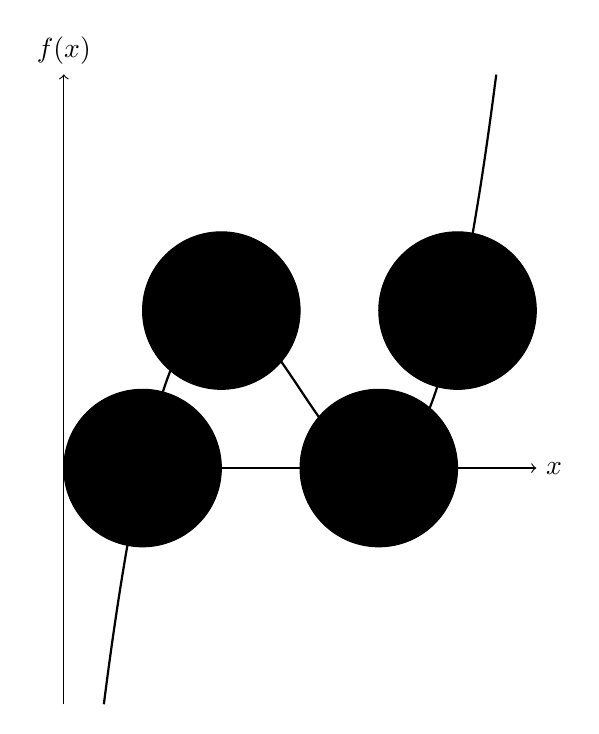
\begin{tikzpicture}
            \draw[->] (0, 0) -- (6, 0) node[right] {$x$};
            \draw[->] (0, -3) -- (0, 5) node[above] {$f(x)$};
            \draw[thick, smooth, samples=100] plot[domain=0.508:5.492] (\x, {((\x)^3 - 9*(\x)^2 + 24*(\x) - 16) / 2});
            \filldraw (2, 2) circle (\pointSize) node[above] {$\left(2; 4\right)$};
            \filldraw (4, 0) circle (\pointSize) node[below] {$\left(4; 0\right)$};
            \filldraw (1, 0) circle (\pointSize) node[below right] {$\left(1; 0\right)$};
            \filldraw (5, 2) circle (\pointSize) node[right] {$\left(5; 4\right)$};
         \end{tikzpicture}
      }
      \caption{Đồ thị của hàm $f(x) = x^3 - 9x^2 + 24x - 16$}
      \label{fig:ham_so_mot_bien:da_thuc:x3_t9x2_24x_t16}
   \end{figure}

   \begin{figure}[H]
      \centering
      \fbox{
         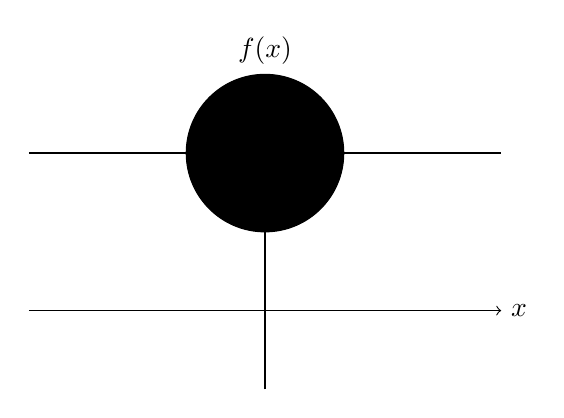
\begin{tikzpicture}
            \draw[->] (-3, 0) -- (3, 0) node[right] {$x$};
            \draw[->] (0, -1) -- (0, 3) node[above] {$f(x)$};
            \draw[thick] plot[domain=-3:3] (\x, {2});
            \filldraw (0, 2) circle (\pointSize) node[above left] {$\left(0; 2\right)$};
         \end{tikzpicture}
      }
      \caption{Đồ thị của hàm $f(x) = 2$}
      \label{fig:ham_so:ham_da_thuc:2}
   \end{figure}

   \begin{figure}[H]
      \centering
      \fbox{
         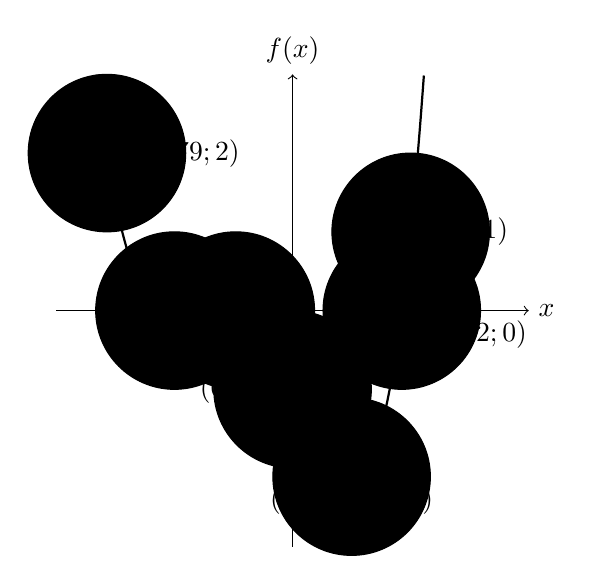
\begin{tikzpicture}
            \draw[->] (-3, 0) -- (3, 0) node[right] {$x$};
            \draw[->] (0, -3) -- (0, 3) node[above] {$f(x)$};
            \draw[thick, smooth, samples=100] plot[domain=-2.491:1.669] (\x, {36*(\x/3)^4 + 28*(\x/3)^3 - 3*(\x/3)^2 - 6*(\x/3) - 1});
            \foreach \x/\y/\xlabel/\ylabel/\pos in {
               -1.5/0/{-0,5}/0/below,
               -0.721/0/{-0,24}/0/above,
               0/-1/0/-1/left,
               0.75/-2.109/{0,25}/{-2,11}/below,
               1.387/0/{0,462}/0/below right,
               -2.357/2/{-0,79}/2/right,
               1.5/1/{0,5}/1/right} {
               \filldraw (\x, \y) circle (\pointSize) node[\pos] {$\left(\xlabel;\ylabel\right)$};
            }
         \end{tikzpicture}
      }
      \caption{Đồ thị của hàm $f(x) = 36x^4 + 28x^3 - 3x^2 - 6x - 1$}
      \label{fig:ham_so:ham_da_thuc:36x4_28x3_t3x2_t6x_t1}
   \end{figure}

   \begin{figure}[H]
      \centering
      \fbox{
         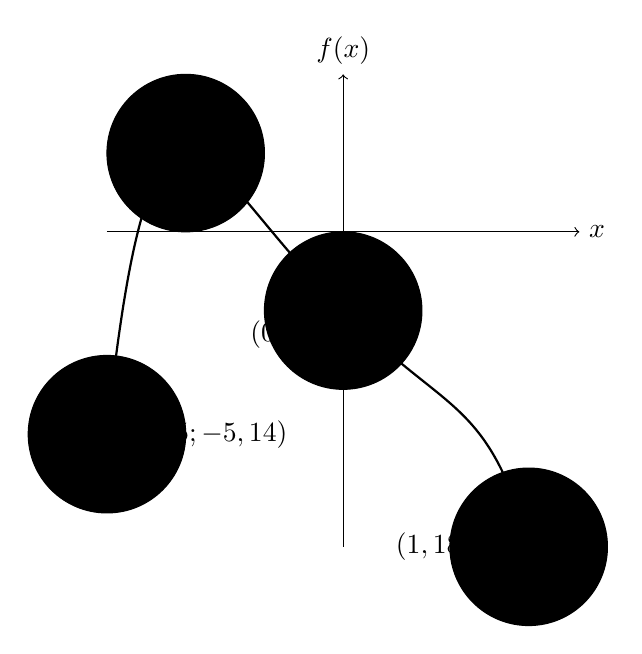
\begin{tikzpicture}
            \draw[->] (-3, 0) -- (3, 0) node[right] {$x$};
            \draw[->] (0, -4) -- (0, 2) node[above] {$f(x)$};
            \draw[thick, smooth, samples=80] plot[domain=-3:2.356] (\x, {(-(\x / 2)^6 + (\x / 2)^2 - 2*(\x) - 2)/2});
            \foreach \x/\y/\xlabel/\ylabel/\pos in {
               -3/-2.570/{-1,5}/{-5,14}/right,
               -2/1/-1/2/above,
               0/-1/0/-1/below left,
               2.356/-4/{1,18}/-8/left} {
               \filldraw (\x, \y) circle (\pointSize) node[\pos] {$\left(\xlabel;\ylabel\right)$};
            }
         \end{tikzpicture}
      }
      \caption{Đồ thị của hàm $f(x) = -x^6 + x^2 - 4x - 2$}
      \label{fig:ham_so:ham_da_thuc:tx6_x2_t4x_t2}
   \end{figure}

   \begin{figure}[H]
      \centering
      \fbox{
         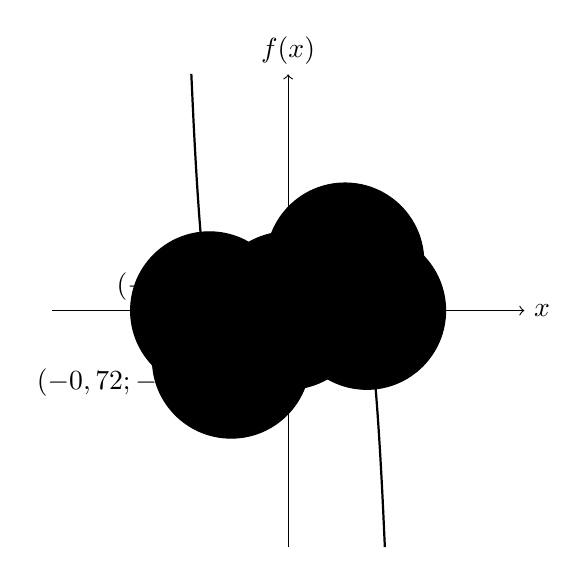
\begin{tikzpicture}
            \draw[->] (-3, 0) -- (3, 0) node[right] {$x$};
            \draw[->] (0, -3) -- (0, 3) node[above] {$f(x)$};
            \draw[thick, smooth, samples=80] plot[domain=-1.229:1.229] (\x, {-(\x)^7 + (\x)});
            \foreach \x/\y/\xlabel/\ylabel/\pos in {
               -1/0/-1/0/above left,
               0/0/0/0/below right,
               1/0/1/0/above right,
               0.723/0.62/{0,72}/{0,62}/above,
               -0.723/-0.62/{-0,72}/{-0,62}/below left}{
                  \filldraw (\x, \y) circle (\pointSize) node[\pos] {$\left(\xlabel;\ylabel\right)$};
            }
         \end{tikzpicture}
      }
      \caption{Đồ thị của hàm $f(x) = -x^7 + x$}
      \label{fig:ham_so:ham_da_thuc:tx7_x}
   \end{figure}
\end{multicols}

\exercise Giải những phương trình sau. Các phương trình đều có ẩn là $x \in \mathbb{R}$.
\begin{multicols}{2}
   \begin{enumerate}
      \item $3x - 7 = 0$;
      \item $x - 9 = 5x + 3$;
      \item $\frac{1}{v}\cdot x - \frac{1}{v} \cdot x_0 = t$, với $v$, $x_0$, $t$ là những tham số thực;
      \item $6x^2 - 5x - 21 = 0$;
      \item $5x^2 - 50x + 125 = 0$;
      \item $x^2 + 2x + 4 = 0$;
      \item $x^2 + 2x + 4 = 8$;
      \item $5x^2 - 20x + 20 = x^2 - 4$;
      \item $\frac{1}{2}kx^2 + \frac{1}{2}mv^2 = \frac{1}{2}kx_0^2$, với $k$, $m$, $v$, $x_0$ là những tham số thực;
      \item $x^3 - \frac{11}{6}\cdot x^2 + x - \frac{1}{6} = 0$;
      \item $2x^3 - 2x^2 + 2x - 2 = 6 + 6x^2$;
      \item $x^4+2x^3-x^2-2x=0$;
      \item $-x^4 -3x^2 = -5$;
      \item $x^4 + 1 = 3x^3 + x^2 + 3x$.
   \end{enumerate}
\end{multicols}

\solution

1. Biến đổi tương đương phương trình để có:
\begin{align*}
   3x - 7 &= 0 \\
   \iff 3x &= 7\\
   \iff x &= \frac{7}{3}.
\end{align*}
Vậy tập nghiệm của phương trình là $\boxed{\displaystyle\left\{\frac{7}{3}\right\}}$.

2. Chuyển số hạng có thừa số $x$ về một phía, và số hạng tự do về phía còn lại để được:
\begin{align*}
   x - 9 &= 5x + 3 \\
   \iff (x - 9) + (9 - 5x) &= (5x + 3) + (9 - 5x) \\ 
   \iff -4x &= 12 \\
   \iff x &= -3.
\end{align*}
Vậy tập nghiệm của phương trình là $\boxed{\displaystyle\left\{-3\right\}}$.

3. Để giải phương trình có chứa tham số, chúng ta cần viết lại ẩn $x$ dưới dạng một biểu thức chỉ chứa tham số và hằng số. Cụ thể,
\begin{align*}
   \frac{1}{v}\cdot x - \frac{1}{v} \cdot x_0 &= t \\
   \iff \frac{x}{v} &= t + \frac{x_0}{v} \\
   \iff x &= vt + x_0.
\end{align*}
Vậy nghiệm của phương trình là $\boxed{\displaystyle\left\{vt + x_0\right\}}$.

4. Nếu như bạn đọc chưa biết, nếu như một đa thức $f(x)$ nhận $x = a$ là nghiệm thì $f(x)$ có thể được viết thành tích của $(x - a)$ nhân một đa thức $g(x)$ với bậc nhỏ hơn $1$ so với $f(x)$. Và nếu $g(x)$ lại có nghiệm $x = b$ thì chúng ta có thể viết $g(x) = (x-b)h(x)$ và qua đó có thể viết lại $f(x) = (x-a)(x-b)h(x)$. Một cách tổng quát nhất, nếu như $f(x)$ là phương trình bậc $n$ có $n$ nghiệm $a_1, a_2, \cdots, a_n$ thì có thể viết lại $$f(x) = A \prod_{i=1}^{n} (x - a_i) = A(x - a_1)(x - a_2)\cdots (x - a_n)$$ với $A$ là hệ số của số hạng có bậc lớn nhất trong đa thức $f(x)$.

Nhẩm nghiệm (bằng cách bấm máy tính) phương trình thì có $x = -\frac{3}{2}$ và $x = \frac{7}{3}$. Chúng ta kì vọng có thể viết lại phương trình dưới dạng $6\left(x - \left(-\frac{3}{2}\right)\right)\left(x - \frac{7}{3}\right) = 0$. Thực vậy, thực hiện phân tích nhân tử để có:
\begin{align*}
   &6x^2 - 5x - 21 = 0 \\
   \iff &6x^2 - 14x + 9x - 21 = 0 \\
   \iff &2x(3x - 7) + 3(3x - 7) = 0 \\
   \iff &(2x + 3)(3x - 7) = 0 \\
   \iff &\left[
      \begin{aligned}
         2x + 3 &= 0 \\
         3x - 7 &= 0
      \end{aligned}
   \right.
   \iff \left[
      \begin{aligned}
         x &= -\frac{3}{2} \\
         x &= \frac{7}{3}
      \end{aligned}
   \right..
\end{align*}
Vậy phương trình có nghiệm là $\boxed{\displaystyle\left\{-\frac{3}{2}; \frac{7}{3}\right\}}$.

5.
\begin{align*}
   5x^2 - 50x + 125 &= 0 \\
   \iff 5\left(x^2 - 10x + 25\right) &= 0 \\
   \iff 5(x - 5)^2 &= 0 \\
   \iff x - 5 &= 0 \\
   \iff x &= 5.
\end{align*}

Vậy tập nghiệm của phương trình có một phần tử duy nhất $\boxed{\displaystyle\left\{5\right\}}$.

6. Với những phương trình liên quan tới đa thức bậc hai không thể nhẩm ngay được nghiệm, chúng ta sẽ sử dụng phương pháp tách bình phương. Với phương trình được cho:
\begin{align}
   x^2 + 2x + 4 &= 0 \nonumber\\ 
   \iff x^2 + 2x + 1 &= -3 \nonumber\\
   \iff (x + 1)^2 &= -3. \label{eq:ham_so_mot_bien:ham_da_thuc:gptdt6}
\end{align}
Một số thực nhân với chính nó sẽ ra một số không âm. Cho nên phương trình \ref{eq:ham_so_mot_bien:ham_da_thuc:gptdt6} không thể đúng. Vậy phương trình \fbox{vô nghiệm} trên tập số thực.

7. 
\begin{align*}
   &x^2 + 2x + 4 = 8 \\ 
   \iff &x^2 + 2x + 1 = 5 \\
   \iff &(x + 1)^2 = 5 \\
   \iff &\left[
      \begin{aligned}
         x + 1 &= \sqrt{5} \\
         x + 1 &= -\sqrt{5}
      \end{aligned}
   \right. \\
   \iff &\left[
      \begin{aligned}
         x &= \sqrt{5} - 1 \\
         x &= -\sqrt{5} - 1
      \end{aligned}
   \right..
\end{align*}
Vậy tập nghiệm của phương trình là $\boxed{\displaystyle\left\{\sqrt{5} - 1; -\sqrt{5} - 1\right\}}$.

8. Phần này tác giả làm khác so với phần 2. Chuyển đổi toàn bộ phương trình về một vế để đưa về dạng phương trình $f(x) = 0$:
\begin{align*}
   &5x^2 - 20x + 20 = x^2 - 4 \\
   \iff &4x^2 - 20x + 24 = 0 \\
   \iff &4\left(x^2 - 5x + 6\right) = 0 \\
   \iff &4\left(x^2 - 2x - 3x + 6\right) = 0 \\
   \iff &4\left(x(x - 2) - 3(x - 2)\right) = 0 \\
   \iff &4(x - 3)(x - 2) = 0 \\
   \iff &\left[
      \begin{aligned}
         x - 3 &= 0 \\
         x - 2 &= 0
      \end{aligned}
   \right. \iff x \in \left\{3; 2\right\}. 
\end{align*}
Vậy phương trình có tập nghiệm $\boxed{\left\{3; 2\right\}}$.

9. Nhân cả hai vế với $2$ để khử phân số trong phương trình:
\begin{align}
   &\frac{1}{2}kx^2 + \frac{1}{2}mv^2 = \frac{1}{2}kx_0^2 \nonumber \\
   \iff &kx^2 + mv^2 = kx_0^2. \label{eq:ham_so_mot_bien:ham_da_thuc:gptdt9}
\end{align}
Xong, thực hiện chuyển vế để giữ thừa số chứa $x^2$ ở một bên, phương trình \ref{eq:ham_so_mot_bien:ham_da_thuc:gptdt9} tương đương với
\begin{align*}
   (\ref{eq:ham_so_mot_bien:ham_da_thuc:gptdt9}) \iff &kx^2 = kx_0^2 - mv^2 \\
   \iff & x^2 = x_0^2 - \frac{mv^2}{k}.
\end{align*}

Với trường hợp $x_0^2 - \frac{mv^2}{k} < 0$ thì phương trình vô nghiệm do $x^2$ không thể âm. Trong trường hợp còn lại, lấy căn bậc hai hai vế để có $$x\in\left\{\sqrt{x_0^2 - \frac{mv^2}{k}}; -\sqrt{x_0^2 - \frac{mv^2}{k}}\right\}.$$ Tại giá trị đặc biệt mà khi $x_0^2 = \frac{mv^2}{k}$ thì tập nghiệm suy biến thành $\left\{0\right\}$.

Vậy, phương trình có nghiệm là 
$$
\boxed{
   \begin{cases}
      \left\{\sqrt{x_0^2 - \frac{mv^2}{k}}; -\sqrt{x_0^2 - \frac{mv^2}{k}}\right\} &\text{ nếu } x_0^2 - \frac{mv^2}{k} \geq 0 \\
      \emptyset &\text{ nếu } x_0^2 - \frac{mv^2}{k} < 0
   \end{cases}.
}
$$

10. Phân tích thừa số với để ý rằng $1$, $\frac{1}{2}$ và $\frac{1}{3}$ là nghiệm:
\begin{align*}
   &x^3 - \frac{11}{6}\cdot x^2 + x - \frac{1}{6} = 0 \\
   \iff &x^3 - x^2 - \frac{5}{6}x^2 + \frac{5}{6}x + \frac{1}{6}x - \frac{1}{6} = 0 \\
   \iff &x^2\left(x - 1\right) - \frac{5}{6}x\left(x - 1\right) + \frac{1}{6}\left(x - 1\right) = 0 \\
   \iff &\left(x - 1\right)\left(x^2 - \frac{5}{6}x + \frac{1}{6}\right) = 0 \\
   \iff &\left(x - 1\right)\left(x^2 - \frac{1}{2}x - \frac{1}{3}x + \frac{1}{6}\right) = 0 \\
   \iff &\left(x - 1\right)\left(x\left(x - \frac{1}{2}\right) - \frac{1}{3}\left(x - \frac{1}{2}\right)\right) = 0 \\
   \iff &\left(x - 1\right)\left(x - \frac{1}{2}\right)\left(x - \frac{1}{3}\right) = 0
\end{align*}
\begin{align*}
   \iff &\left[
      \begin{aligned}
         x - 1 &= 0 \\
         x - \frac{1}{2} &= 0 \\
         x - \frac{1}{3} &= 0
      \end{aligned}
   \right. \\
   \iff &\left[
      \begin{aligned}
         x &= 1 \\
         x &= \frac{1}{2} \\
         x &= \frac{1}{3}
      \end{aligned}
   \right..
\end{align*}
Cuối cùng, như chúng ta đã dự đoán, phương trình có nghiệm là $\boxed{\displaystyle\left\{1; \frac{1}{2}; \frac{1}{3}\right\}}$.

11. Có một cách là chuyển phương trình về một vế rồi nhẩm nghiệm. Dưới đây, tác giả sẽ trình bày một góc nhìn khác để giải bài toán này.
\begin{align}
   2x^3 - 2x^2 + 2x - 2 &= 6 + 6x^2 \nonumber\\
   \iff \left(2x^3 + 2x\right) - \left(2x^2 + 2\right) &= 6x^2 + 6 \nonumber\\
   \iff 2x\left(x^2 + 1\right) - 2\left(x^2 + 1\right) &= 6\left(x^2 + 1\right) \nonumber\\
   \iff \left(2x - 2\right)\left(x^2 + 1\right) &= 6\left(x^2 + 1\right). \label{eq:ham_so_mot_bien:ham_da_thuc:gptdt11}
\end{align}
Để ý rằng, do $x^2 \geq 0$ nên $x^2 + 1 \geq 1 > 0$. Chúng ta đã chỉ ra rằng $x^2 + 1 \neq 0$, và qua đó, chúng ta có thể an toàn chia hai vế của \ref{eq:ham_so_mot_bien:ham_da_thuc:gptdt11} cho $x^2 + 1$ để có:
\begin{align*}
   2x - 2 &= 6 \\
   \iff x &= 4.
\end{align*}
Vậy phương trình có nghiệm là $\boxed{\displaystyle\left\{4\right\}}$.

12. Dễ dàng thấy được có thể phân tích thừa số của đa thức được cho như sau:
\begin{align*}
   x^4 + 2x^3 - x^2 -2x &= 0 \\
   \iff x(x^3 + 2x^2 - x - 2) &= 0 \\
   \iff x(x + 2)(x^2 - 1) &= 0 \\
   \iff x(x + 2)(x - 1)(x + 1) &= 0.
\end{align*}

Chia làm $4$ trường hợp: $\left[
   \begin{aligned}
      x &= 0 \\
      x + 2&= 0 \\
      x - 1 &= 0 \\
      x + 1 &= 0
   \end{aligned}
\right.$ và giải từng trường hợp một để có $x \in \left\{0; -2; 1; -1\right\}$.

Vậy phương trình có bộ nghiệm là $\boxed{\displaystyle\left\{0; -2; 1; -1\right\}}$.

\def\varPhu {\textit{付}}

13. Đặt $\varPhu = x^2$ để đưa từ đa thức bậc bốn về đa thức bậc hai như sau:
\begin{align*}
   -x^4 - 3x^2 &= -5 \\
   \iff -\varPhu^2 - 3\varPhu &= -5 \\
   \iff \varPhu^2 + 3\varPhu - 5 &= 0.
\end{align*}

Giải phương trình bậc hai này bằng công thức nghiệm, chúng ta có:
$$
\left[
   \begin{aligned}
      \varPhu &= \frac{-3 + \sqrt{3^2 - 4 \cdot (-5)}}{2} = \frac{-3 + \sqrt{29}}{2} \\
      \varPhu &= \frac{-3 - \sqrt{3^2 - 4 \cdot (-5)}}{2} = \frac{-3 - \sqrt{29}}{2}
   \end{aligned}
\right..
$$ Tuy nhiên, do $\varPhu = x^2 \geq 0$ nên $\varPhu$ chỉ có thể nhận giá trị $\frac{-3 + \sqrt{29}}{2}$, và qua đó $x^2 = \frac{-3 + \sqrt{29}}{2}$. Vậy phương trình có nghiệm là $x \in \boxed{\left\{\sqrt{\frac{-3 + \sqrt{29}}{2}}; -\sqrt{\frac{-3 + \sqrt{29}}{2}}\right\}}$.

14. Bài tập này dành cho những bạn chuyên toán thuần hơn là về ứng dụng. Nhận thấy rằng $x = 0$ không là nghiệm của phương trình. Chia cả hai vế của phương trình cho $x^2 \neq 0$ để có 
\begin{equation}
   x^2 + \frac{1}{x^2} = 3x + 1 + \frac{3}{x}. 
   \label{eq:ham_so_mot_bien:da_thuc:gptdt14}
\end{equation}
Đặt $y = x + \frac{1}{x}$, bình phương hai vế để có $y^2 = \left(x + \frac{1}{x}\right)^2 = x^2 + \frac{1}{x^2} + 2$ hay $x^2 + \frac{1}{x^2} = y^2 - 2$. Thay vào \ref{eq:ham_so_mot_bien:da_thuc:gptdt14}, chúng ta có:
\begin{align*}
   y^2 - 2 &= 3y + 1 \\
   \iff y^2 - 3y - 3 &= 0.
\end{align*}
Giải phương trình này bằng công thức nghiệm:
\begin{equation}   
   \left[
      \begin{aligned}
         y &= \frac{3 + \sqrt{3^2 - 4 \cdot (-3)}}{2} = \frac{3 + \sqrt{21}}{2} \\
         y &= \frac{3 - \sqrt{3^2 - 4 \cdot (-3)}}{2} = \frac{3 - \sqrt{21}}{2}
      \end{aligned}
   \right..\label{eq:ham_so_mot_bien:da_thuc:gpt14y}
\end{equation}

Giải phương trình $x + \frac{1}{x} = y$. Nếu chúng ta nhân cả tử và mẫu với $x$, chúng ta sẽ có phương trình với đa thức bậc hai theo ẩn $x$: $$x^2 - yx + 1 = 0.$$ Cũng dùng công thức nghiệm để giải phương trình này để được:
$$
\left[
   \begin{aligned}
      x &= \frac{y + \sqrt{y^2 - 4}}{2} \\
      x &= \frac{y - \sqrt{y^2 - 4}}{2}
   \end{aligned}
\right..
$$

Do $x \in \mathbb{R}$ nên giá trị trong dấu khai căn $y^2 - 4$ phải không nhỏ hơn $0$. Kiểm tra hai giá trị $y$ tìm được từ \ref{eq:ham_so_mot_bien:da_thuc:gpt14y}, chúng ta thấy $y = \frac{3 + \sqrt{21}}{2}$ thỏa mãn điều kiện này. Thay thế trực tiếp để tìm được tập nghiệm của phương trình.

Cuối cùng, chúng ta có được $x \in$ \fbox{$\displaystyle\left\{\frac{3+\sqrt{21}+\sqrt{14 + 6\sqrt{21}}}{2}; \frac{3+\sqrt{21}-\sqrt{14 + 6\sqrt{21}}}{2}\right\}$}.

\exercise Giải các bất phương trình sau. Các bất phương trình đều có ẩn là $x \in \mathbb{R}$.

\begin{multicols}{2}
   \begin{enumerate}
      \item $4x + 7 < 0$;
      \item $-8x - 16 > 0$;
   \end{enumerate}
\end{multicols}

\solution


\exercise Xác định tập giá trị của những hàm sau:
\begin{multicols}{2}
   \begin{enumerate}
      \item $f(x) = 0$;
      \item $f(x) = 10x - 20$;
      \item $f(x) = x^2 + 2x + 3$;
      \item $f(x) = x^4 + 2x^2 + 3$.
   \end{enumerate}
\end{multicols}

\solution

1. Theo định nghĩa, do hàm chỉ trả về kết quả là $0$ nên tập giá trị của $f$ là $\boxed{\left\{0\right\}}$.

2. Nhận thấy mọi giá trị $y \in \mathbb{R}$ đều có thể là kết quả của $f$ do:
$$f\left(\frac{y}{10} + 2\right) = 10 \left(\frac{y}{10} + 2\right) - 20 = y.$$
Vậy tập giá trị của $f$ là $\boxed{\mathbb{R}}$.

3. Theo đồ thị \ref{fig:ham_so_mot_bien:da_thuc:x2_2x_3}, chúng ta thấy được $f$ nhận mọi giá trị trong khoảng $\left[2; \infty\right)$. Về mặt đại số, biến đổi $f$ để có:
$$f(x) = x^2 + 2x + 3 = (x + 1)^2 + 2 \geq 2.$$

Điều này khẳng định là nếu $y = f(x)$ thì $y \geq 2$. Tuy nhiên, nó chưa khẳng định là $y \geq 2$ là đủ để có $x$ thỏa mãn $y = f(x)$. Để làm được điểu này, chúng ta phải viết phương trình $y = f(x)$ và tìm một $x$ là nghiệm của phương trình đó. Với $y\geq 2$, chúng ta đặt $x = -1 + \sqrt{y - 2}$ và thực hiện tính $f(x)$:
\begin{align*}
   f\left(-1 + \sqrt{y - 2}\right) &= \left(-1 + \sqrt{y - 2}\right)^2 + 2\left(-1 + \sqrt{y - 2}\right) + 3 \\
   &= \left(1 - 2\sqrt{y - 2} + y - 2\right) + \left(- 2 + 2\sqrt{y - 2}\right) + 3 \\
   &= y.
\end{align*}
Qua đó, chúng ta kết luận với $y \geq 2$ thì tồn tại $x$ để $y = f(x)$.

Vậy tập giá trị của $f$ là $\boxed{\left[2; \infty\right)}$.

4. Bình phương của một số thì luôn không âm. Cho nên $x^2 \geq 0$ và $x^4 = x^2 \times x^2$ là tích của hai số không âm thì là một số không âm. Do đó $x^4 + 2x^2 + 3 \geq 3$.

Ngược lại, mọi số thực $y$ từ $3$ trở lên đều có thể có một giá trị $x$ sao cho $x^4 + 2x^2 + 3 = y$. Do $y \geq 3$ nên
\begin{align*}
   y - 2 &\geq 1 \\
   \iff \sqrt{y - 2} &\geq 1 \\
   \iff \sqrt{y - 2} - 1 &\geq 0.
\end{align*}
Qua đó, chúng ta có thể lấy khai căn và đặt $x = \sqrt{\sqrt{y - 2} - 1}$. Khi này, thực hiện tương tự như đã làm ở phần 3 để có $f(x) = y$. Vậy tập giá trị của $f$ là $\boxed{\left[3; \infty\right)}$.


